\documentclass[border=0.2cm]{report}
 
% Required packages
\usepackage{tikz}
\usetikzlibrary{shapes,positioning}
\usepackage{hyperref} % for url link
\hypersetup{
    colorlinks=true,
    linkcolor=blue,
    filecolor=magenta,      
    urlcolor=blue,
}
\usepackage[norelsize, ruled, lined, boxed, commentsnumbered]{algorithm2e}
\usepackage{physics} % for gradient
\usepackage{optidef} % equation number
\usepackage{bm} % for bold fonts

\usepackage{amsfonts} % contains \mathbb{R}
\newcommand{\R}{\mathbb{R}} % create command \R from \mathbb{R}
 
\title{Evolutionary Algorithms (EA)}
\author{Gergő Bonnyai}
\date{\today}

\begin{document}
\maketitle

\tableofcontents
\listoffigures

\clearpage

\chapter{Differential Evolution (DE)}
\section{Story}
\section{Pseudo code}
\section{Flowchart}

\chapter{Evolutionary Strategy (ES)}
\section{Story}
\section{Pseudo code}
\section{Flowchart}

\chapter{Cuckoo Search (CS)}
\section{Story}
\section{Pseudo code}
\section{Flowchart}

\chapter{Artificial Bee Colony (ABC)}
\section{Story}
\section{Pseudo code}
\section{Flowchart}

\chapter{Particle Swarm Optimization (PSO)}
\section{Story}
\section{Pseudo code}
\section{Flowchart}

\chapter{Whale Optimization Algorithm (WOA)}
\section{Story}
\section{Pseudo code}
\section{Flowchart}

\chapter{Grey Wolf Optimization (GWO)}
\section{Story}
\section{Pseudo code}
\section{Flowchart}

\chapter{Flower Pollination Algorithm (FPA)}
\section{Story}
\section{Pseudo code}
\section{Flowchart}

\chapter{Firefly Algorithm (FA)}
\section{Story}
\section{Pseudo code}
\section{Flowchart}

\chapter{Black Hole Algorithm (BHA)}
\section{Story}

BHA \cite{bha1, bha2} heuristic approach was introduced in 2012. The analogy is to create a random population of stars in the search space, the one with the best fitness value is considered as the black hole. The black hole gives a direction for every star's movement in all iterations. The stars are moving towards the black hole in a random way. After movement if the fitness value of a star is higher than the fitness value of the black hole, then this star becomes the black hole. Furthermore another mechanism is involved to make a balance between exloration and exploitation, according to that if a star cross the event horizon (defined distance from the black hole) then the black hole swallows it. Technically the star loose it's actual position and being redistributed randomly in the search space. Hence a new star is born to keep the population constant. \\

\noindent
Let $X=\{x_1,x_2,\ldots,x_N\}$ population of stars, where $N$ is the population size and $x_i \in \R^D$.
$f: \R^{D}\to\R^1$ is the fitness function and $fitness_i=f(x_i)$ is the fitness value of $x_i$.\\
\noindent
Movement of stars towards the black hole:
\begin{equation}\label{eqn_bha_step}
x_i(t+1)=x_i(t)+rand*(x_{BH}-x_i(t))
\end{equation}
where $x_i(t)$ is the location of the ith star at iteration $t$, and $x_{BH}$ is the black hole. $x_{BH}: fitness_{BH}=\displaystyle \max_{i=1,\dots, N}f(x_i)$. $rand \in U(0, 1)$, where $U$ stands for uniform distribution.\\
\noindent
Radius of the event horizon is calculated as follows:
\begin{equation}\label{eqn_bha_event_horizon}
Event Horizon=\frac{fitness_{BH}}{\sum\limits_{i=1}^N fitness_i}
\end{equation}



\section{Pseudo code}

\begin{algorithm}[H]
\caption{Black Hole Algorithm}
 
 \Begin{
 Set $N$: population size, $T$: number of iterations \\
 Initialize random population of stars $X=\{x_1,x_2,\ldots,x_N\}$, \\
 Calculate fitness values $fitness_i$, determine the black hole $x_{BH}$, \\
 \While{$t<T$ or Stopping criteria not met}{
  \For{$i \gets 1 \textrm{ to } N$}{
      Update location of star $x_i$ by Equation \ref{eqn_bha_step} \\
      Check search space \\
      Calculate $fitness_i=f(x_i)$ \\
      \If{$fitness_i<fitness_{BH}$}{
      $x_{BH}=x_i$ \\
      $fitness_{BH}=fitness_i$ \\
      Calculate $Event Horizon$ by Equation \ref{eqn_bha_event_horizon}
      }
      \Else{
      \If{$\norm{x_{BH}-x_{i}}<Event Horizon$}{
      Reinitialize $x_i$ randomly within the search space
      }
      }
    } 
    Check Stopping Criteria \\
    $t=t+1$
 }
 }
\end{algorithm}

\section{Flowchart}

\begin{figure}[ht]
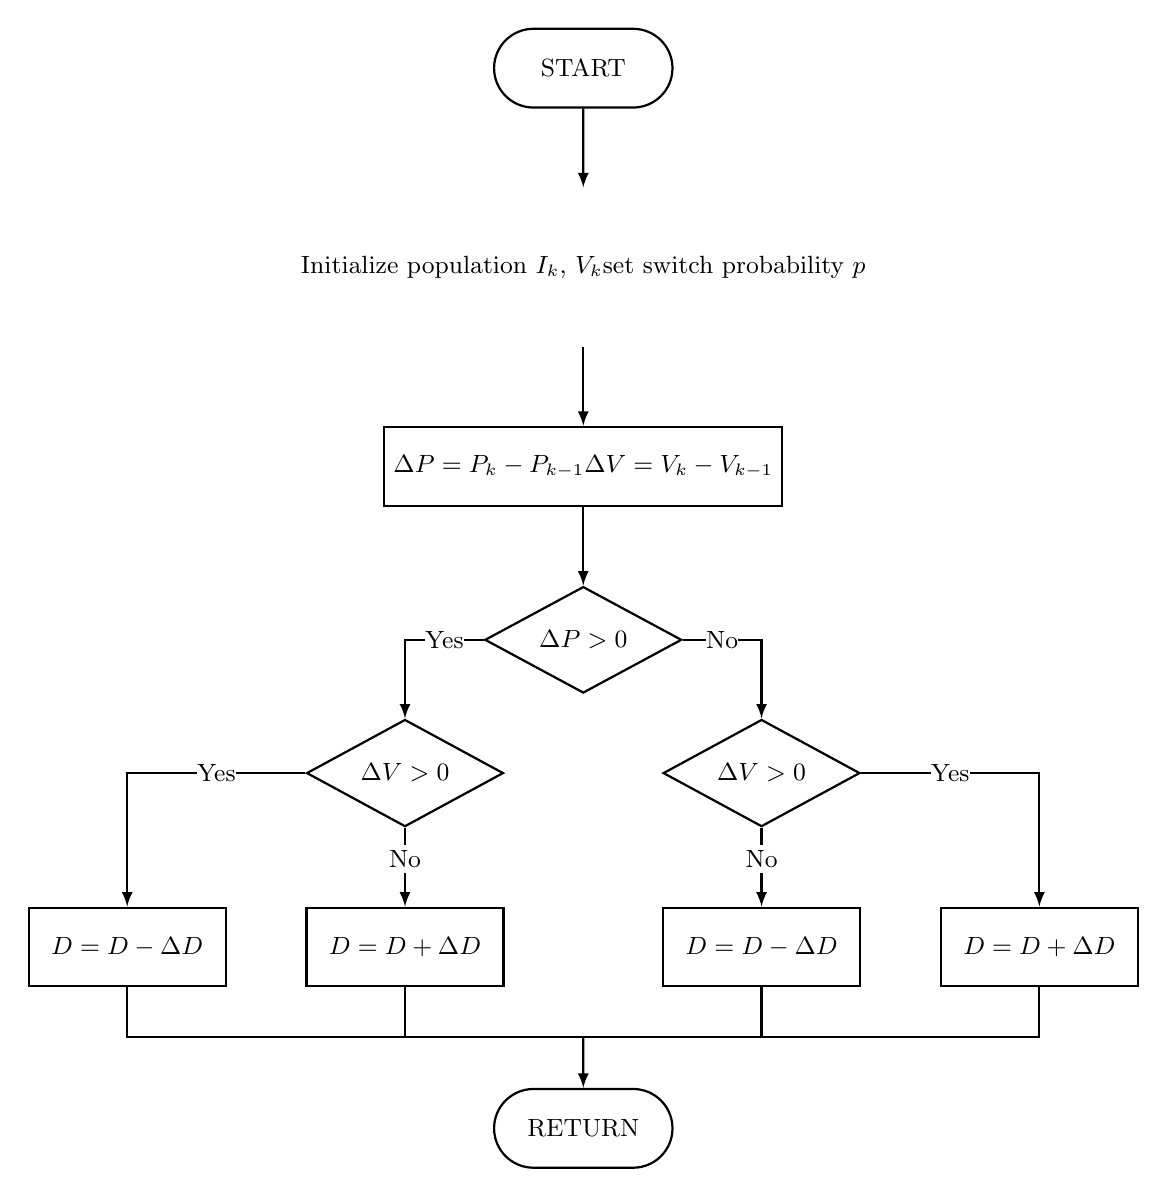
\begin{tikzpicture}[font=\small,thick]
 
% Start block
\node[draw,
    rounded rectangle,
    minimum width=2.5cm,
    minimum height=1cm] (block1) {START};
 
% Voltage and Current Measurement
\node[rectangle, %draw,
    below=of block1,
    minimum width=3.5cm,
    minimum height=2cm
] (block2) { Initialize population $I_k$, $V_k$ \\
set switch probability $p$  };
 
% Power and voltage variation
\node[draw,
    below=of block2,
    minimum width=3.5cm,
    minimum height=1cm
] (block3) { $\Delta P=P_k-P_{k-1}$ \\ $\Delta V=V_k-V_{k-1}$};
 
% Conditions test
\node[draw,
    diamond,
    below=of block3,
    minimum width=2.5cm,
    inner sep=0] (block4) { $\Delta P>0$};
 
\node[draw,
    diamond,
    below left=of block4,
    minimum width=2.5cm,
    inner sep=0] (block5) { $\Delta V>0$};
 
\node[draw,
    diamond,
    below right=of block4,
    minimum width=2.5cm,
    inner sep=0] (block6) { $\Delta V>0$};
 
% Increase and Decrease duty cycle
\node[draw,
    below=of block5,
    minimum width=2.5cm,
    minimum height=1cm] (block7) { $D=D+\Delta D$};
 
\node[draw,
    left=of block7,
    minimum width=2.5cm,
    minimum height=1cm] (block8) { $D=D-\Delta D$};
 
\node[draw,
    below=of block6,
    minimum width=2.5cm,
    minimum height=1cm] (block9) { $D=D-\Delta D$};
 
\node[draw,
    right=of block9,
    minimum width=2.5cm,
    minimum height=1cm] (block10) { $D=D+\Delta D$};
 
% Return block
\node[draw,
    rounded rectangle,
    below=5cm of block4,
    minimum width=2.5cm,
    minimum height=1cm,] (block11) { RETURN};
 
\node[coordinate,below=4.35cm of block4] (block12) {};
 
 
% Arrows
\draw[-latex] (block1) edge (block2)
    (block2) edge (block3)
    (block3) edge (block4);
 
\draw[-latex] (block4) -| (block5)
    node[pos=0.25,fill=white,inner sep=0]{Yes};
 
\draw[-latex] (block4) -| (block6)
    node[pos=0.25,fill=white,inner sep=0]{No};
 
\draw[-latex] (block5) edge node[pos=0.4,fill=white,inner sep=2pt]{No}(block7)
    (block5) -| (block8)
        node[pos=0.25,fill=white,inner sep=0]{Yes};
 
\draw[-latex] (block6) edge node[pos=0.4,fill=white,inner sep=2pt]{No}(block9)
    (block6) -| (block10)
        node[pos=0.25,fill=white,inner sep=0]{Yes};
 
\draw (block7) |- (block12);
\draw (block9) |- (block12);
\draw (block8) |- (block7|-block12);
\draw (block10) |- (block9|-block12);
\draw[-latex] (block12) -- (block11);
 
\end{tikzpicture}

\caption{Flowchart of Flower Pollination Algorithm (FPA)}
\end{figure}



\begin{thebibliography}{9}
\bibitem{bha1} 
Hatamlou, A., 2012. \textit{Black hole: A new heuristic optimization approach for data clustering.} Information sciences, 2012: p. 175-184. 

\bibitem{bha2} 
M. Farahmandian, A. Hatamlou, 2015. \textit{Solving optimization problems using black hole algorithm} Journal of Advanced Computer Science \& Technology, 2015: p. 68-74. \\
Link: \url{https://www.sciencepubco.com/index.php/JACST/article/view/4094/1621}\\

\end{thebibliography}


\end{document}